\chapter{Signaling Pathway Activities Improve Prognosis for Breast Cancer}
\label{chap:hipathia}
%\minitoc

\begin{chapabstract}

\textrm{{\bf Abstract:}} With the advent of high-throughput technologies for genome-wide expression profiling, a large number of methods have been proposed to discover gene-based signatures as biomarkers to guide cancer prognosis. However, it is often difficult to interpret the list of genes in a prognostic signature regarding the underlying biological processes responsible for disease progression or therapeutic response. A particularly interesting alternative to gene-based biomarkers is mechanistic biomarkers, derived from signaling pathway activities, which are known to play a key role in cancer progression and thus provide more informative insights into cellular functions involved in cancer mechanism. In this chapter, we demonstrate that a pathway-level feature, such as the activity of signaling circuits, outperform conventional gene-level features in prediction performance in breast cancer prognosis. We also show that the proposed classification scheme can even suggest, in addition to relevant signaling circuits related to disease outcome, a list of genes that do not code for signaling proteins whose contribution to cancer prognosis potentially supplements the mechanisms detected by pathway analysis. This study is under submission as joint work with Marta R. Hidalgo, Cankut \c{C}ubuk, Alicia Amadoz, Jos\'{e} Carbonell-Caballero, Jean-Philippe Vert, Joaqu\'{i}n Dopazo \cite{Jiao2017Signaling}.
\linebreak
\vskip 0.1in
\noindent \textrm{{\bf R�sum�:}}

\end{chapabstract}


\section{Introduction}
\label{sec5:intro}

Breast cancer is one of the most common malignancy for women and breast cancer prognosis is currently one of the leading problems of great interest. The advent of high-throughput platforms for gene expression profiling motivates the popular trend of using molecular biomarkers for clinical decision making regarding prognosis improvement assisting therapeutic strategies. It has been widely recognized as a very promising yet challenging problem to extract potentially valuable information from genomic data. The relatively small number of clinical samples, the inherent measurement noise in high-throughput experimental data and the heterogeneity across patients make it demanding to detect reliable biomarkers.














Over the past decades, many efforts have been addressed to the identification of gene-based signatures to predict  patient prognosis using gene expression data [1-4]. Despite the success of its use, gene expression signatures have not been exempt of problems [5, 6]. Specifically, one major drawback of multi-gene biomarkers is that they often lack proper interpretation in terms of mechanistic link to the fundamental cell processes responsible for disease progression or therapeutic response [7, 8]. Actually, it is increasingly recognized that complex traits, such as disease or drug response, are better understood as alterations in the operation of functional modules caused by different combinations of gene perturbations [9-11]. To address this inherent complexity different methodologies have tried to exploit several functional module conceptual representations, such as protein interaction networks or pathways, to interpret gene expression data within a systems biology context  [10, 12-14]. Actually, it has recently been shown that the pathway-level representation generates clinically relevant stratifications and outcome predictors for glioblastoma and colorectal cancer [15] and also breast cancer [16]. Moreover, mathematical models of the activity of a pathway have demonstrated a significantly better association to poor prognosis in neuroblastoma patients than the activity of their constituent genes, including MICN, a conventional biomarker [17]. This observation has recently been extended to other cancers [18] and to the prediction of drug effects [19].

Given that the inferred activity of the pathway should be closely related to its cellular mechanism for disease progression, its use to guide cancer prognosis seems promising. Recently, a number of pathway activity inference methods have been proposed [18, 20-22]. Here, we use the canonical circuit activity analysis method, which has demonstrated to have a superior performance [18] finding significant associations of specific circuit activities, directly responsible for triggering the prominent cancer hallmarks [23], to patient survival. This method recodes gene expression values into measurements of signaling circuit activities that ultimately account for cell responses to specific stimuli. Such activity values can be considered multigenic mechanistic biomarkers that can be used as features for cancer prognosis. 
We demonstrate that the activity of signaling circuits yields comparable or even better prediction in breast cancer prognosis than the expression of individual genes, while detected mechanistic biomarkers enjoy the compelling advantage of readily available interpretation in terms of the corresponding cellular functions they trigger. Moreover, we show that the proposed prediction scheme can even suggest, in addition to interesting signaling circuits related to disease outcome, a list of prognostic genes that do not code for signaling proteins whose contribution to cancer prognosis potentially supplements the mechanism included in the pathways modeled. 

We demonstrate that the activity of signaling circuits yields comparable or even better prediction in breast cancer prognosis than the expression of individual genes, while detected mechanistic biomarkers enjoy the compelling advantage of readily available interpretation in terms of the corresponding cellular functions they trigger. Moreover, we show that the proposed prediction scheme can even suggest, in addition to interesting signaling circuits related to disease outcome, a list of prognostic genes that do not code for signaling proteins whose contribution to cancer prognosis potentially supplements the mechanism included in the pathways modeled. 










Over the past decades several groups have pursued to identify gene-based signatures to classify patients with good or poor prognosis with gene expression data of breast tumors from large cohorts \cite{VantVeer2002Gene, Paik2004multigene, Wang2005Gene, Sotiriou2009Gene, Reis-Filho2011Gene}. Despite the vast success of such traditional analysis, although many detected prognostic genes are known to be related to cell cycle and proliferation for instance, multi-gene biomarkers often lack proper interpretation in terms of mechanistic link to the fundamental cell processes responsible for disease progression or therapeutic response.

To address this problem, there is a pressing need to develop methods that integrate \textit{a priori} known biological information in the process of genomic data analysis. It is well understood that cell signaling is a system of within-cell communication and signal transduction process between gene products, mostly proteins, that coordinates cell activities to perceive and correctly respond to microenvironment, resulting in signaling pathways that form a particular type of functional gene modules and play a key role in disease progression (Figure \ref{fig:cellsignaling}). Consequently as a tempting solution to the limitation of conventional analysis at the level of individual genes, analysis at the level of pathways renders great interest in providing informative insights into cellular functions that facilitates understanding of the disease mechanism. Furthermore, oncogenic pathways are usually dysregulated at different levels along cancer progression, and thus pathway-guided prognosis has the potential to achieve comparable or even better performance compared to traditional gene-based prognosis. The recent demonstration by \cite{Fey2015Signaling} constitutes an elegant confirmation of this concept that the activity of a pathway presents a significantly better association to poor prognosis in neuroblastoma patients than the activity of their constituent genes (among them MICN, a conventional biomarker). As another example, \cite{Drier2013Pathway} introduced Pathifier, an algorithm that infers pathway deregulation levels for each tumor sample on the basis of expression data, and showed that the pathway-level representation generates clinically relevant stratifications and outcome predictors for glioblastoma and colorectal cancer.

\begin{figure}[!htbp]
	\centering
	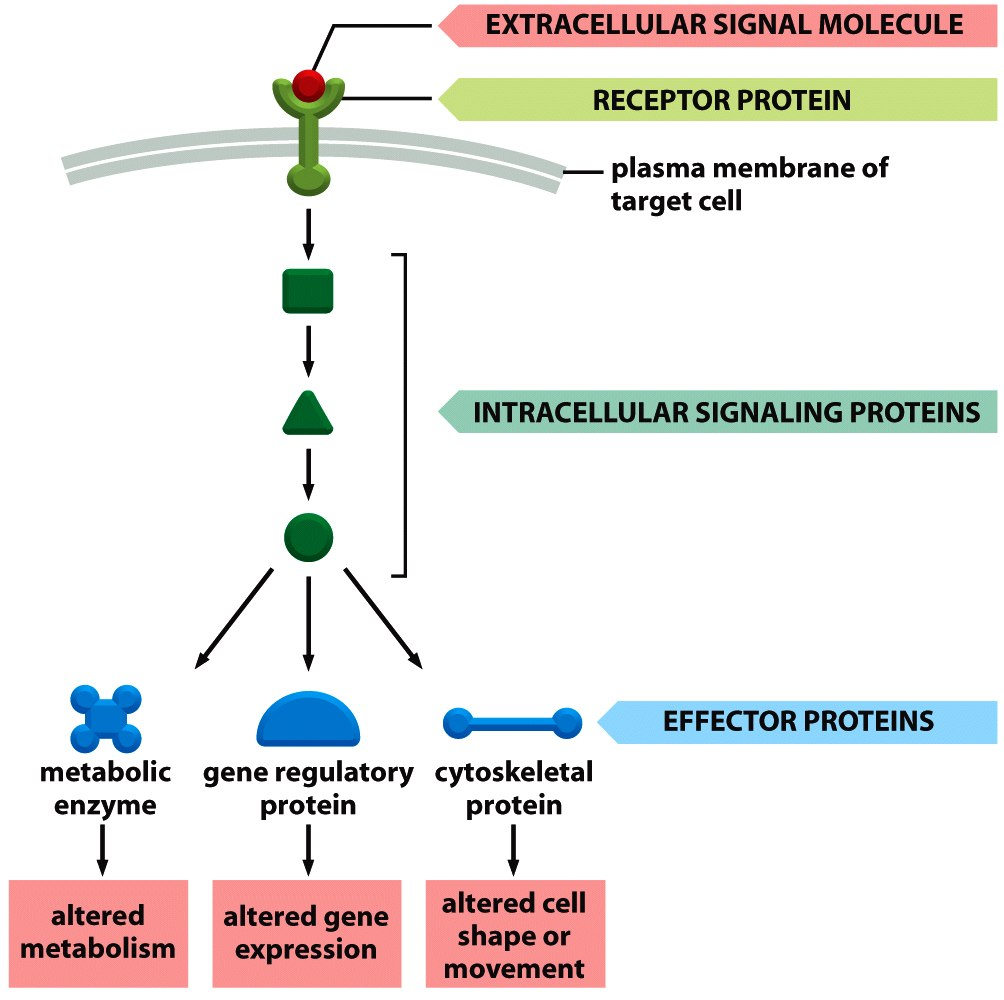
\includegraphics[width=0.6\textwidth]{ch5hipathia/figure/signaling_pathway}
	\caption{An illustration of cell signaling process. Typically the signal transduction begins at receptor proteins that receive molecular stimuli from cell microenvironment and ends at effector proteins that execute specific actions in response to the stimulation.}
	\label{fig5:cellsignaling}
\end{figure}

To use signaling pathways to guide cancer prognosis, we first need a way to infer the activity level of a given pathway based on the expression of the constituent genes. The inferred activity of the pathway should be closely related to its cellular mechanism for disease progression. Recently, a number of pathway activity inference methods have been proposed \cite{Jacob2012More, Martini2013Along, Li2015Subpathway, Hidalgo2016High}, and in this study we apply the canonical circuit activity analysis (CCAA) method introduced by \cite{Hidalgo2016High}. In fact, CCAA is a method that estimates the level of activity within a pathway by modeling cell signaling process in order to recode gene expression values into measurements that ultimately account for cell responses caused by the activity of the pathway. Essentially the CCAA method computes an activity value for each stimulus-response sub-pathway, called canonical circuit, within signaling pathways. The canonical circuits which associate naturally with cell functionalities can be considered as pathway-level mechanistic features that are modularized from multigenic signatures, and their activity values connected to the activation or deactivation of specific cellular functions thus provide quantitative clues to understand disease mechanisms when related to phenotypes of interest. In particular, \cite{Hidalgo2016High} showed that the CCAA method can be used to find significant association of specific pathway activities to patient survival, among which several are directly responsible for triggering the prominent cancer hallmarks \cite{Hanahan2011Hallmarks}. This verifies that the CCAA method is capable of capturing pathway activities and thus cell processes involved in disease outcome.

In this study, we take one step further and study the prognostic power of the pathway-level mechanistic features whose activity levels are inferred by the CCAA method. We demonstrate that the activity of signaling circuits yields comparable or even better prediction in breast cancer prognosis than the expression of individual genes, while detected pathway-level biomarkers enjoy the compelling advantage of readily available interpretation in terms of the corresponding cellular functions. Finally we show that the proposed prediction scheme can even suggest, in addition to interesting signaling circuits related to disease outcome, a list of prognostic genes that do not code for signaling proteins whose contribution to cancer prognosis potentially supplements the mechanism perceived by pathway analysis. All experiments are produced with \texttt{R} and codes are available via \url{https://github.com/YunlongJiao/hipathiaCancerPrognosis}.

